\documentclass[notitlepage]{article}

\usepackage{etoolbox}
\patchcmd{\thebibliography}{\chapter*}{\section*}{}{}

\title{A Quantum \texttt{popcount} Circuit for Sieving}
\author{Martin R.~Albrecht, Eamonn W.~Postlethwaite}
\date{\today}

\usepackage{amsmath}
\usepackage{amsfonts}
\usepackage{amssymb}

\usepackage{braket}
\usepackage{subcaption}
\usepackage{graphicx}

\usepackage{array}
\usepackage{booktabs}
\renewcommand{\arraystretch}{1}

\usepackage{tikz}

\usepackage{algorithm}
\usepackage{algpseudocode}

\usepackage{amsthm}
\newtheorem*{thm}{Theorem}
\newtheorem*{lem}{Lemma}
\theoremstyle{definition}
\newtheorem*{mydef}{Definition}
\newtheorem*{heu}{Heuristic}

\definecolor{niceorange}{HTML}{FFDD00}
\usepackage[color=niceorange]{todonotes}
\usepackage{xspace}
\newcommand{\malb}[2][inline]{\todo[#1]{\textbf{malb:} #2}\xspace}

\usepackage{geometry}

\begin{document}

\maketitle

\section*{Introduction and Preliminaries}

Using the adders of~\cite{cuccaro2004new,Takahashi:2008:FQC} we build reversible circuits that take as input bitstring representatives of two lattice vectors, take a bitwise \texttt{CNOT},\malb[]{Why not call it XOR?} determine the Hamming weight of the outcome and further determine whether this Hamming weight is smaller than some bound.
This exact operation is the most frequently used operation in state of the art lattice sieving techniques.

Throughout qubits $a_{i}$ are ancillae and are initialised as $\ket{0}$.
The $v_{i}, w_{i} \in \{0, 1\}, i \in \{0, \dots, d - 1\}$ form the bitstring representatives of lattice vectors $v, w$.
These are calculated as the signs of the entries of $v$ and $w$, i.e.~a negative entry is mapped to $0$ and a positive or zero entry to $1$.
This provides a lossy sketch of the lattice vectors under consideration.
The \texttt{CNOT} gate is written as \texttt{CNOT}$(x, y) = (x, x \oplus y)$.
Gates labelled \texttt{add} are all either the adder of~\cite{cuccaro2004new} or the adder of~\cite{Takahashi:2008:FQC}.

To sum two $\ell$ bit numbers, the adder of~\cite{cuccaro2004new} takes $2\ell + 2$ inputs, the topmost and bottommost are ancillae and those inbetween are the interleaved bits of the numbers to be added.
More precisely let $x = x_{\ell-1}\dots x_{0}$ and $y = y_{\ell-1}\dots y_{0}$ be two numbers to be added represented in binary, then \texttt{add}$(a_{0}, x_{0}, y_{0}, \dots, x_{\ell-1}, y_{\ell-1}, a_{1}) = (a_{0}, s_{0}, y_{0}, \dots, s_{\ell-1}, y_{\ell-1}, s_{\ell})$ with $s_{i}$ as bit $i$ of the sum.
In particular the first ancillary remains $\ket{0}$ but the second contains the final carry.

The adder of~\cite{Takahashi:2008:FQC} functions similarly but instead requires $2\ell + O(\ell/\log_{2}\ell)$ inputs, that is $O(\ell/\log_{2}\ell)$ ancillae.
While this adder requires more ancillae, it has an optimal depth of $O(\log\ell)$ compared to the depth $O(\ell)$ of the above adder.

We need some number, linear in $d$, of the \texttt{add} gates described above.

The notation $s^{i\dots j}_{k}$ in Figure~\ref{fig:naive_popcnt} denotes bit $k$ of the sum (over the integers)
\[
    \displaystyle\sum\limits_{l=i}^{j}{v_{l} \oplus w_{l}}.
\]
Finally the \texttt{OR} gate in Figure~\ref{subfig:naive_popcnt3} consumes an ancillary, \texttt{OR}$(a, x, y) = (a \oplus (xy), x\vee y, y)$.

A reduction between $v$ and $w$ is likely if the sum of bits (considered as Integers) of $v_{i} \oplus w_{i}$ is less than some bound, here $2^{k}, k \in \mathbb{Z}_{\geq 1}$.
Let the bit length of this sum be denoted $n = \lfloor\log_{2}d\rfloor + 1$.
We therefore take a (non exclusive) \texttt{OR} over the $n - k$ high bits of the sum and reject pair $(v, w)$ for further testing if we receive a $\ket{1}$.
We require some number, linear in $n$, of the \texttt{OR} gates described above.
An example with $d = 4, k = 1$, using the adder of~\cite{cuccaro2004new} is given in Figure~\ref{fig:naieve_popcnt}.\malb[]{In subfigure (c), is that a three-way XOR?}

\begin{figure}
    \begin{subfigure}{.3\textwidth}
        \centering
        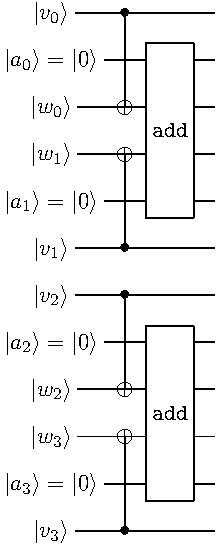
\includegraphics{popcnt_sieve_pt1}
        \caption{The \texttt{CNOT}s and the first round of addition.}\label{subfig:naive_popcnt1}
    \end{subfigure}
    \dots
    \begin{subfigure}{.3\textwidth}
        \centering
        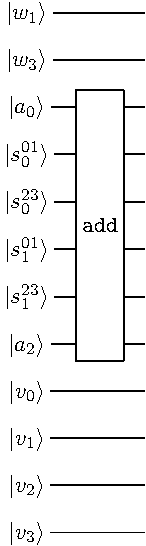
\includegraphics{popcnt_sieve_pt2}
        \caption{Another round of addition.}\label{subfig:naive_popcnt2}
    \end{subfigure}
    \dots
    \begin{subfigure}{.3\textwidth}
        \centering
        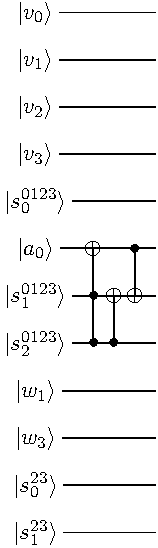
\includegraphics{popcnt_sieve_pt3}
        \caption{An \texttt{OR}, the centre qubit of the three determines the outcome.}\label{subfig:naive_popcnt3}
    \end{subfigure}
    \caption{A simple quantum circuit for determining whether a specific \texttt{popcount} is greater than a given bound.}\label{fig:naive_popcnt}
\end{figure}

\section*{Depth, Width and Size of Circuit with~\cite{cuccaro2004new} adder}

We require at most $d$ ancillae as inputs to the \texttt{add} gates, with one definitely remaining in the state $\ket{0}$.
Furthermore, we require $O(n)$ ancillae for the \texttt{OR} gates.
In terms of $d$ this is $d + O(\log_{2}d)$ ancillae. The width of the circuit is therefore $3d + O(\log_{2}d)$, $2d$ of which represent $v, w$.

The $d$ \texttt{CNOT}s require\dots\ $d$ \texttt{CNOT} gates.
There are $d/2^{i}$ \texttt{add} gates which add two $i$ bit numbers together, for $i \in \{1, \dots, \lceil \log_{2}d\rceil\}$. Each has a number, linear in $i$, of \texttt{Toffoli} and \texttt{CNOT} gates. Therefore the number of such gates required is $O(d)$.\malb[]{I don't follow here}
The $O(n)$ \texttt{OR} gates require $O(n)$ \texttt{CNOT} and \texttt{Toffoli} gates, or $O(\log_{2}d)$ of both.
In total the circuit has $O(d)$ \texttt{CNOT} and \texttt{Toffoli} gates.\malb[]{Is that what you mean by ``size'' in the Figure? Maybe rename to gates}

The depth of the circuit is $O\left({(\log_{2}d)}^{2}\right)$. This is calculated as
\[
    \displaystyle\sum\limits_{i = 1}^{\lceil\log_{2}d\rceil}{O(i)} + \displaystyle\sum\limits_{i = 1}^{\lceil \log_{2}n\rceil}{O(1)} = O\left({(\log_{2} d)}^{2}\right) + O\left(\log_{2}(\log_{2}d)\right) = O\left({(\log_{2} d)}^{2}\right).
\]

\section*{Depth, Width and Size of Circuit with~\cite{Takahashi:2008:FQC} adder}

The size of this circuit is the same, namely $O(d)$ \texttt{Toffoli} and \texttt{CNOT} gates.
The ancillae requirements are higher, although still linear.
Indeed, in~\cite{Takahashi:2008:FQC}, for large $n$ they give the number of ancillae to be $3n/\log n - O(\log n)$, and so the total number of ancillae required for the \texttt{add} gates is less than
\[
    \displaystyle\sum\limits_{i = 1}^{\lceil \log_{2}d\rceil}{\frac{3id}{2^{i}}} \leq 6d.
\]
Therefore we require at most $6d + O(\log_{2}d)$ ancillae for a total width of at most $8d + O(\log_{2}d)$.
Finally the depth of the circuit is calculated as\malb[]{What does the \({t = \lceil\log_{2}d\rceil}\) notation mean?}
\begin{align*}
    \displaystyle\sum\limits_{i = 1}^{\lceil \log_{2}d\rceil}{O(\log i)} + \displaystyle\sum\limits_{i = 1}^{\lceil \log_{2}n\rceil}{O(1)} &= O\left.\left(\frac{1}{2}\log(2\pi) + t(\log t - 1) + O(\log t)\right)\right|_{t = \lceil\log_{2}d\rceil} + O\left(\log_{2}(\log_{2}d)\right)\\
    &= O\left(\log_{2}d\left(\log_{2}(\log_{2}d)\right)\right) + O\left(\log_{2}(\log_{d}d)\right)\\
    &= O\left(\log_{2}d\left(\log_{2}(\log_{2}d)\right)\right),
\end{align*}
where the first sum is evaluated using a truncation of the Euler--Maclaurin formula. % chktex 8
As expected this is a smaller depth than above.
These results are summarised in Figure~\ref{tab:GDW}.

\begin{figure}
    \centering
    \begin{tabular}{lrrr}
        \toprule
                                    & size      & depth & width\\
        \midrule
        \cite{cuccaro2004new}       & $O(d)$    & $O\left({(\log_{2}d)}^{2}\right)$ & $3d + O(\log_{2}d)$\\ % chktex 2
        \cite{Takahashi:2008:FQC}   & $O(d)$    & $O\left(\log_{2}d\left(\log_{2}(\log_{d}d)\right)\right)$ & $8d + O(\log_{2}d)$\\ % chktex 2
        \bottomrule
    \end{tabular}
    \caption{A summary of the size, depth and width of circuit when using different adders.}\label{tab:GDW}
\end{figure}

\bibliographystyle{alpha}
\bibliography{local}

\end{document}

%%% Local Variables:
%%% mode: latex
%%% TeX-master: t
%%% End:
